\chapter{Réalisation, tests et résultats}

\section{Introduction}

Ce chapitre présente les résultats obtenus après la mise en œuvre de la solution, ainsi que les vérifications réalisées sur ses principales composantes. L’objectif est de montrer l’apport concret de la solution par rapport au processus initial basé principalement sur les fichiers Excel.

L’évaluation porte sur des éléments mesurables : le temps d’exécution du pipeline, les volumes chargés dans MySQL, les situations détectées par le moteur de validation, les réponses des APIs, ainsi que la restitution des données à travers Power BI, l’application mobile et le portail back-office.

Ce chapitre permet ainsi de vérifier que les données issues du terrain peuvent être préparées, centralisées, contrôlées puis exploitées dans une chaîne plus structurée de suivi des opérations de merchandising.

\section{Démarche d’évaluation des résultats}

La démarche d’évaluation repose sur des preuves observables. Chaque composante de la solution est analysée à travers une question simple, liée à son rôle dans le suivi global.

\begin{tcolorbox}[
    colback=gray!4,
    colframe=black!60,
    title=\textbf{Questions d’évaluation retenues},
    fonttitle=\bfseries,
    arc=2mm,
    boxrule=0.6pt,
    left=6pt,
    right=6pt,
    top=6pt,
    bottom=6pt
]
\textbf{Apport data-driven :} la solution permet-elle de passer d’un suivi manuel basé sur Excel à une exploitation centralisée, traçable et décisionnelle des données terrain ?\\[0.35em]
\textbf{Pipeline Data Engineering :} le pipeline permet-il d’automatiser et de tracer la préparation des données ?\\[0.35em]
\textbf{Base MySQL :} les données nécessaires au suivi merchandising sont-elles centralisées ?\\[0.35em]
\textbf{Moteur de validation :} les règles produisent-elles des situations exploitables pour la revue interne ?\\[0.35em]
\textbf{Services backend :} les APIs respectent-elles la séparation entre consultation mobile et back-office ?\\[0.35em]
\textbf{Interfaces et dashboards :} les résultats sont-ils restitués sous une forme lisible et exploitable ?
\end{tcolorbox}

Les axes d’évaluation retenus correspondent aux principaux objectifs de la solution : apport data-driven, centralisation des données, traçabilité des traitements, contrôle métier, séparation des APIs, restitution décisionnelle et consultation applicative.

\subsection{Axes d’évaluation retenus}

Les axes d’évaluation retenus permettent de vérifier si la solution apporte une amélioration réelle par rapport au fonctionnement initial basé sur les fichiers Excel. L’évaluation ne se limite donc pas à vérifier que les outils fonctionnent, mais cherche à mesurer leur contribution à une exploitation plus structurée, traçable et décisionnelle des données terrain.

Les principaux axes retenus sont les suivants :

\begin{itemize}
    \item \textbf{Apport data-driven :} passage d’un suivi manuel basé sur Excel vers une exploitation centralisée, traçable et décisionnelle des données terrain.
    \item \textbf{Centralisation des données :} transformation des fichiers \textit{Data Dump} et \textit{Coverage} en données structurées dans MySQL.
    \item \textbf{Traçabilité des traitements :} suivi des exécutions, des statuts et des journaux à travers Prefect.
    \item \textbf{Contrôle métier :} production de situations exploitables à partir des règles de validation OSA et GPS.
    \item \textbf{Exposition contrôlée :} séparation entre les APIs de consultation mobile et les APIs internes du back-office.
    \item \textbf{Restitution des résultats :} exploitation des données à travers Power BI, l’application mobile et le portail back-office.
\end{itemize}

Ces axes constituent la base de lecture des résultats présentés dans la suite du chapitre.

\subsection{Indicateurs et formules de calcul}

Les indicateurs retenus dans ce chapitre permettent d’interpréter les résultats obtenus après la mise en œuvre de la solution. Ils ne sont pas présentés comme des définitions théoriques, mais comme des repères de calcul utilisés pour mesurer l’apport de la solution : gain de temps, couverture d’exécution, déviation, disponibilité produit et visibilité en rayon.

\subsubsection{Gain de temps mesurable}

Le gain de temps permet d’évaluer l’écart entre le processus manuel initial et l’exécution automatisée du pipeline. Il constitue un indicateur important, car il traduit directement l’impact opérationnel de l’automatisation.

La logique de calcul retenue est la suivante :

\[
\mathrm{Gain\ de\ temps} =
T_{\mathrm{avant}} - T_{\mathrm{apres}}
\]

\[
\text{Taux de réduction} =
\frac{T_{\mathrm{avant}} - T_{\mathrm{apres}}}
{T_{\mathrm{avant}}}
\times 100
\]

où \(T_{\mathrm{avant}}\) représente le temps estimé du processus manuel, et \(T_{\mathrm{apres}}\) le temps mesuré après automatisation.

\subsubsection{Couverture d’exécution}

Dans la solution développée, la couverture d’exécution mesure le niveau de réalisation du périmètre planifié. Une visite en déviation est considérée comme un magasin couvert, car elle correspond à une exécution réelle sur le terrain.

La logique de calcul retenue est la suivante :

\[
N_{\mathrm{visited\_stores}} =
N_{\mathrm{executed\_visits}} + N_{\mathrm{deviation\_visits}}
\]

\[
\mathrm{Execution\ Coverage\ Rate} =
\frac{N_{\mathrm{visited\_stores}}}
{N_{\mathrm{planned\_visits}}}
\times 100
\]

Cette formule permet de distinguer les magasins réellement couverts des magasins uniquement planifiés.

\subsubsection{Déviation d’exécution}

La déviation est calculée par rapport aux magasins effectivement visités. Ce choix évite de mélanger les magasins non visités avec les magasins visités dans une condition particulière.

\[
\mathrm{Deviation\ Rate} =
\frac{N_{\mathrm{deviation\_visits}}}
{N_{\mathrm{visited\_stores}}}
\times 100
\]

Cet indicateur complète le taux de couverture, car il permet d’identifier la part des visites couvertes nécessitant une attention particulière.

\subsubsection{Indicateurs OSA et SOS}

Les indicateurs OSA et SOS complètent l’analyse de l’exécution terrain. Ils permettent d’évaluer la disponibilité produit et la visibilité en rayon à partir des données collectées en magasin.

\[
\mathrm{OSA} =
\frac{N_{\mathrm{available\_products}}}
{N_{\mathrm{checked\_products}}}
\times 100
\qquad
\mathrm{SOS} =
\frac{V_{\mathrm{reported}}}
{V_{\mathrm{total}}}
\times 100
\]

Dans la solution, ces indicateurs sont exploités sous forme synthétique dans les dashboards et dans l’application mobile, sans exposer les détails internes du moteur de validation.

\section{Résultats du pipeline Data Engineering}

Le pipeline Data Engineering constitue le premier résultat concret de la solution. Il permet de transformer les fichiers \textit{Data Dump} et \textit{Coverage}, exportés depuis le portail Smollan, en données structurées, historisées et exploitables dans la base MySQL \dbtable{unilever\_db}.

L’évaluation de cette partie repose sur trois éléments principaux : l’exécution automatisée du pipeline, les volumes chargés dans MySQL et l’apport obtenu par rapport à l’exploitation manuelle des fichiers Excel.

\subsection{Automatisation et traçabilité de l’exécution}

L’automatisation du pipeline remplace une partie des manipulations manuelles par une exécution structurée, mesurable et traçable. Chaque traitement est intégré dans un flux Prefect, avec un statut d’exécution, une durée mesurée et des journaux associés.

La figure \ref{fig:prefect_completed_run_time} présente un exemple d’exécution complète du flux journalier.

\begin{figure}[H]
    \centering
    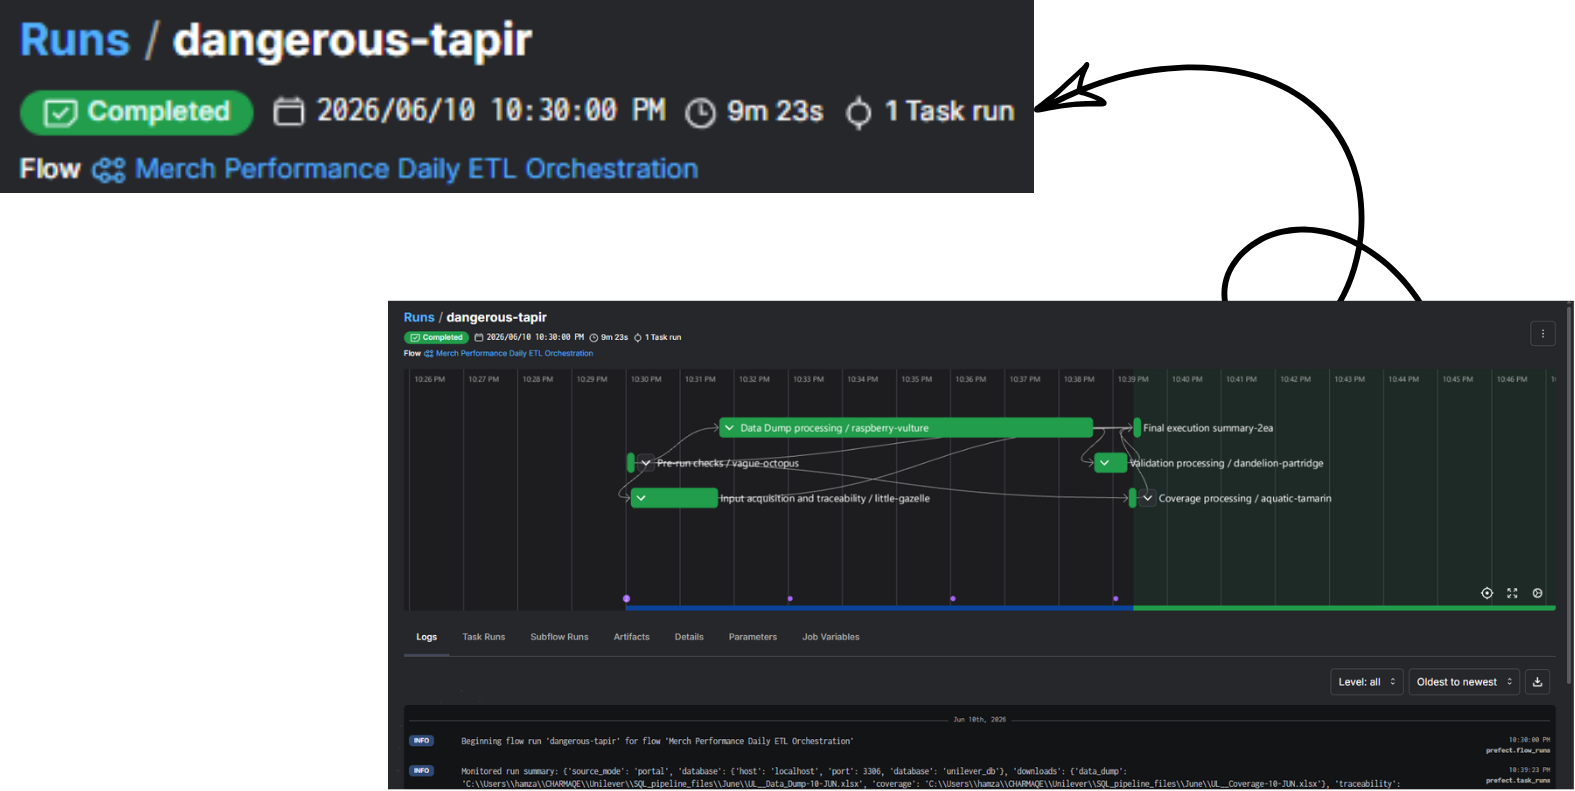
\includegraphics[width=1\textwidth]{figures/results/prefect_completed_run_time.png}
    \caption{Exécution mesurée du pipeline journalier dans Prefect}
    \label{fig:prefect_completed_run_time}
\end{figure}

Dans l’exécution présentée, le flux \textit{Merch Performance Daily ETL Orchestration} s’est terminé avec le statut \textit{Completed}. La durée totale observée est de 9 minutes et 23 secondes. Cette valeur constitue un résultat mesurable, car elle permet d’évaluer le temps nécessaire pour préparer les données à travers la chaîne automatisée.

Ce résultat montre que la solution met en place un processus contrôlé et réutilisable. En cas d’échec, les statuts et les journaux d’exécution facilitent l’identification de l’étape concernée, au lieu de rechercher l’origine du problème dans plusieurs fichiers ou traitements isolés.

\subsection{Centralisation des données dans MySQL}

La centralisation des données dans MySQL constitue un résultat essentiel du pipeline. L’objectif n’était pas seulement de stocker les fichiers exportés depuis le portail Smollan, mais de transformer les fichiers \textit{Data Dump} et \textit{Coverage} en données structurées, interrogeables et réutilisables par les autres composants de la solution.

\begin{figure}[H]
    \centering
    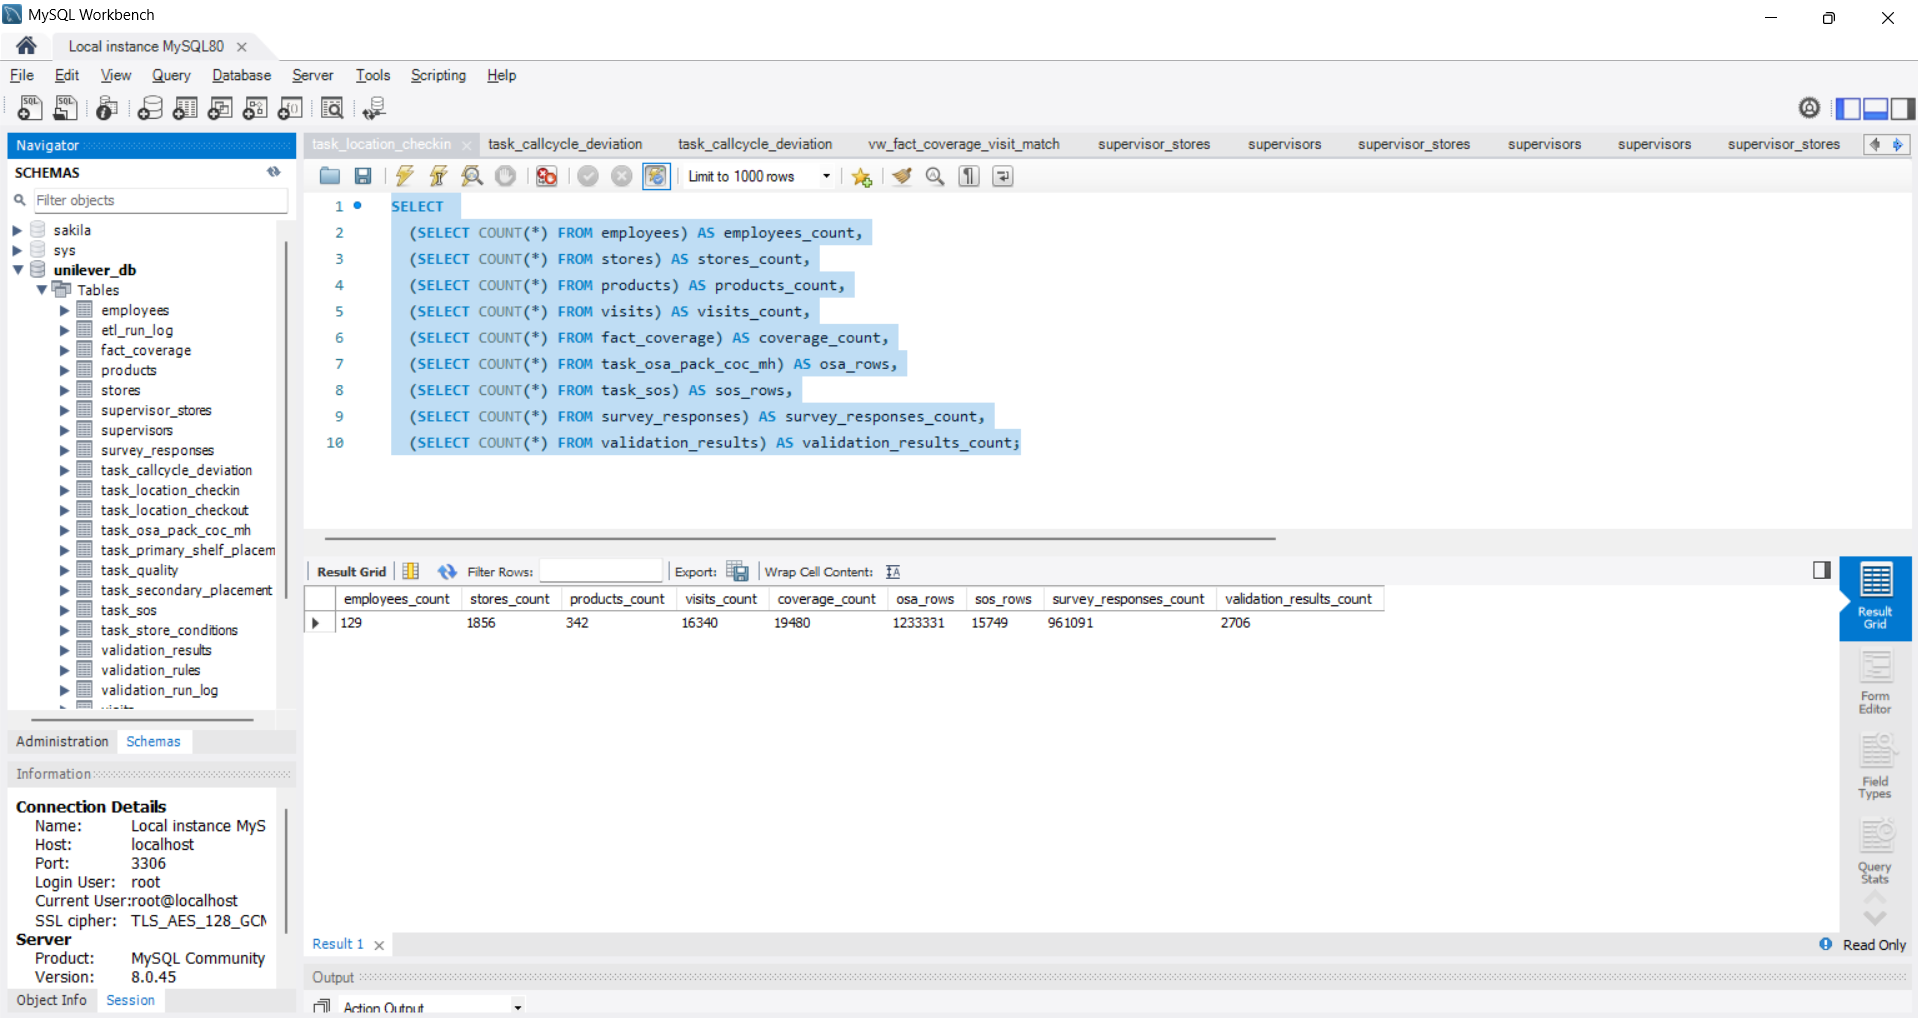
\includegraphics[width=1\textwidth]{figures/results/mysql_loaded_data_summary.png}
    \caption{Synthèse des principales données chargées dans MySQL}
    \label{fig:mysql_loaded_data_summary}
\end{figure}

\textbf{Résultat mesuré :} après exécution du pipeline, la base \dbtable{unilever\_db} contient les principales familles de données nécessaires au suivi merchandising : référentiels, visites terrain, couverture, réponses normalisées, tâches détaillées et résultats de validation.

La synthèse affichée dans MySQL met notamment en évidence le chargement de \textbf{129 employés}, \textbf{1\,856 magasins}, \textbf{342 produits}, \textbf{16\,340 visites} et \textbf{19\,480 lignes de couverture}. Elle montre également le volume important des données détaillées, avec plus de \textbf{1,2 million de lignes OSA} et plus de \textbf{960\,000 réponses normalisées}.

\textbf{Interprétation :} ces volumes montrent que la solution ne traite pas uniquement des indicateurs agrégés. Elle centralise des données détaillées à forte granularité, ce qui justifie l’utilisation d’un pipeline automatisé et d’une base relationnelle. Une exploitation manuelle dans Excel devient difficile à maintenir sur ce volume, notamment lorsqu’il faut croiser les visites, la couverture, les réponses terrain et les résultats de validation.

\textbf{Valeur apportée :} la base MySQL devient une référence commune pour les différentes couches de la solution. Les mêmes données structurées peuvent être exploitées par le moteur de validation, les APIs backend, les dashboards Power BI, l’application mobile et le portail back-office. Cette centralisation améliore la cohérence des résultats et permet de conserver un historique exploitable des opérations de merchandising.

\subsection{Apport par rapport à l’exploitation Excel}

L’un des apports les plus mesurables du pipeline Data Engineering concerne la réduction de la dépendance aux traitements manuels réalisés sous Excel. Dans le processus initial, les fichiers \textit{Data Dump} et \textit{Coverage} devaient être extraits, préparés, croisés et exploités pour produire les reportings internes et les reportings destinés au client.

D’après l’observation du processus existant, la préparation du suivi interne pouvait prendre environ 1h30, tandis que la préparation des reportings client nécessitait environ 1h supplémentaire. Le temps de préparation quotidien mesurable pouvait donc atteindre environ 2h30, soit 150 minutes.

Avec la solution développée, l’exécution automatisée du pipeline observée dans Prefect a été réalisée en 9 minutes et 23 secondes. Ce temps couvre l’enchaînement des traitements nécessaires à la préparation des données structurées et à l’exécution des règles de validation.

Le gain de temps mesurable peut donc être estimé de la manière suivante :

\[
T_{\mathrm{manuel}} = 1h30 + 1h00 = 150 \ \mathrm{minutes}
\]

\[
T_{\mathrm{pipeline}} = 9 \ \mathrm{minutes} \ 23 \ \mathrm{secondes}
\approx 9{,}38 \ \mathrm{minutes}
\]

\[
\mathrm{Gain\ de\ temps} =
T_{\mathrm{manuel}} - T_{\mathrm{pipeline}}
= 150 - 9{,}38
= 140{,}62 \ \mathrm{minutes}
\]

\[
\text{Taux de réduction} =
\frac{T_{\mathrm{manuel}} - T_{\mathrm{pipeline}}}
{T_{\mathrm{manuel}}}
\times 100
\approx 93{,}7\%
\]

\begin{tcolorbox}[
    colback=green!4,
    colframe=green!45!black,
    title=\textbf{Gain réel mesuré},
    fonttitle=\bfseries,
    arc=2mm,
    boxrule=0.6pt,
    left=6pt,
    right=6pt,
    top=6pt,
    bottom=6pt
]
Le passage d’un traitement manuel estimé à \textbf{150 minutes} vers une exécution automatisée de \textbf{9 minutes et 23 secondes} représente un gain d’environ \textbf{140 minutes}, soit une réduction estimée à \textbf{93,7\%} du temps de préparation.
\end{tcolorbox}

Cette estimation reste volontairement prudente, car elle ne comptabilise pas entièrement le temps consacré aux vérifications manuelles détaillées, notamment l’analyse logique des réponses OSA et la recherche des incohérences GPS.

Au-delà du temps gagné, l’apport du pipeline concerne aussi la fiabilité et la traçabilité du processus. Les mêmes règles de transformation peuvent être rejouées de manière stable, les exécutions sont historisées dans Prefect, et les résultats sont centralisés dans MySQL. La solution ne remplace donc pas seulement un traitement manuel par un traitement plus rapide ; elle transforme les fichiers Excel en une chaîne data-driven structurée, mesurable et exploitable par les autres composants de la solution.

\section{Résultats du moteur de validation}

Le moteur de validation constitue la couche de contrôle interne de la solution. Son objectif est de transformer les données terrain centralisées dans MySQL en situations ciblées, exploitables par les équipes internes pour la revue métier. Il ne remplace pas la décision humaine, mais il permet d’orienter l’analyse vers les cas nécessitant une attention particulière.

\subsection{Résultat global obtenu}

L’exécution du moteur de validation a généré \textbf{460 situations de validation}, réparties entre \textbf{457 situations OSA} et \textbf{3 situations GPS}. La règle OSA concerne le périmètre MT et vise à identifier les réponses inhabituelles par rapport au comportement observé au niveau de la bannière. La règle GPS concerne le périmètre GT et permet de détecter les écarts de localisation significatifs sur des visites répétées.

\textbf{Interprétation :} ce résultat montre que le moteur agit comme un filtre métier. Au lieu de parcourir manuellement un volume important de lignes OSA ou de visites GPS, les équipes internes disposent d’une liste ciblée de situations à analyser.

\subsection{Structure détaillée des situations détectées}

Les situations détectées ne sont pas stockées uniquement sous forme d’un code de règle ou d’un message d’alerte. Chaque ligne de la table \dbtable{validation\_results} contient également un champ \dbtable{details\_json}, qui conserve les éléments de contexte utilisés pour interpréter la situation détectée.

\begin{figure}[H]
    \centering
    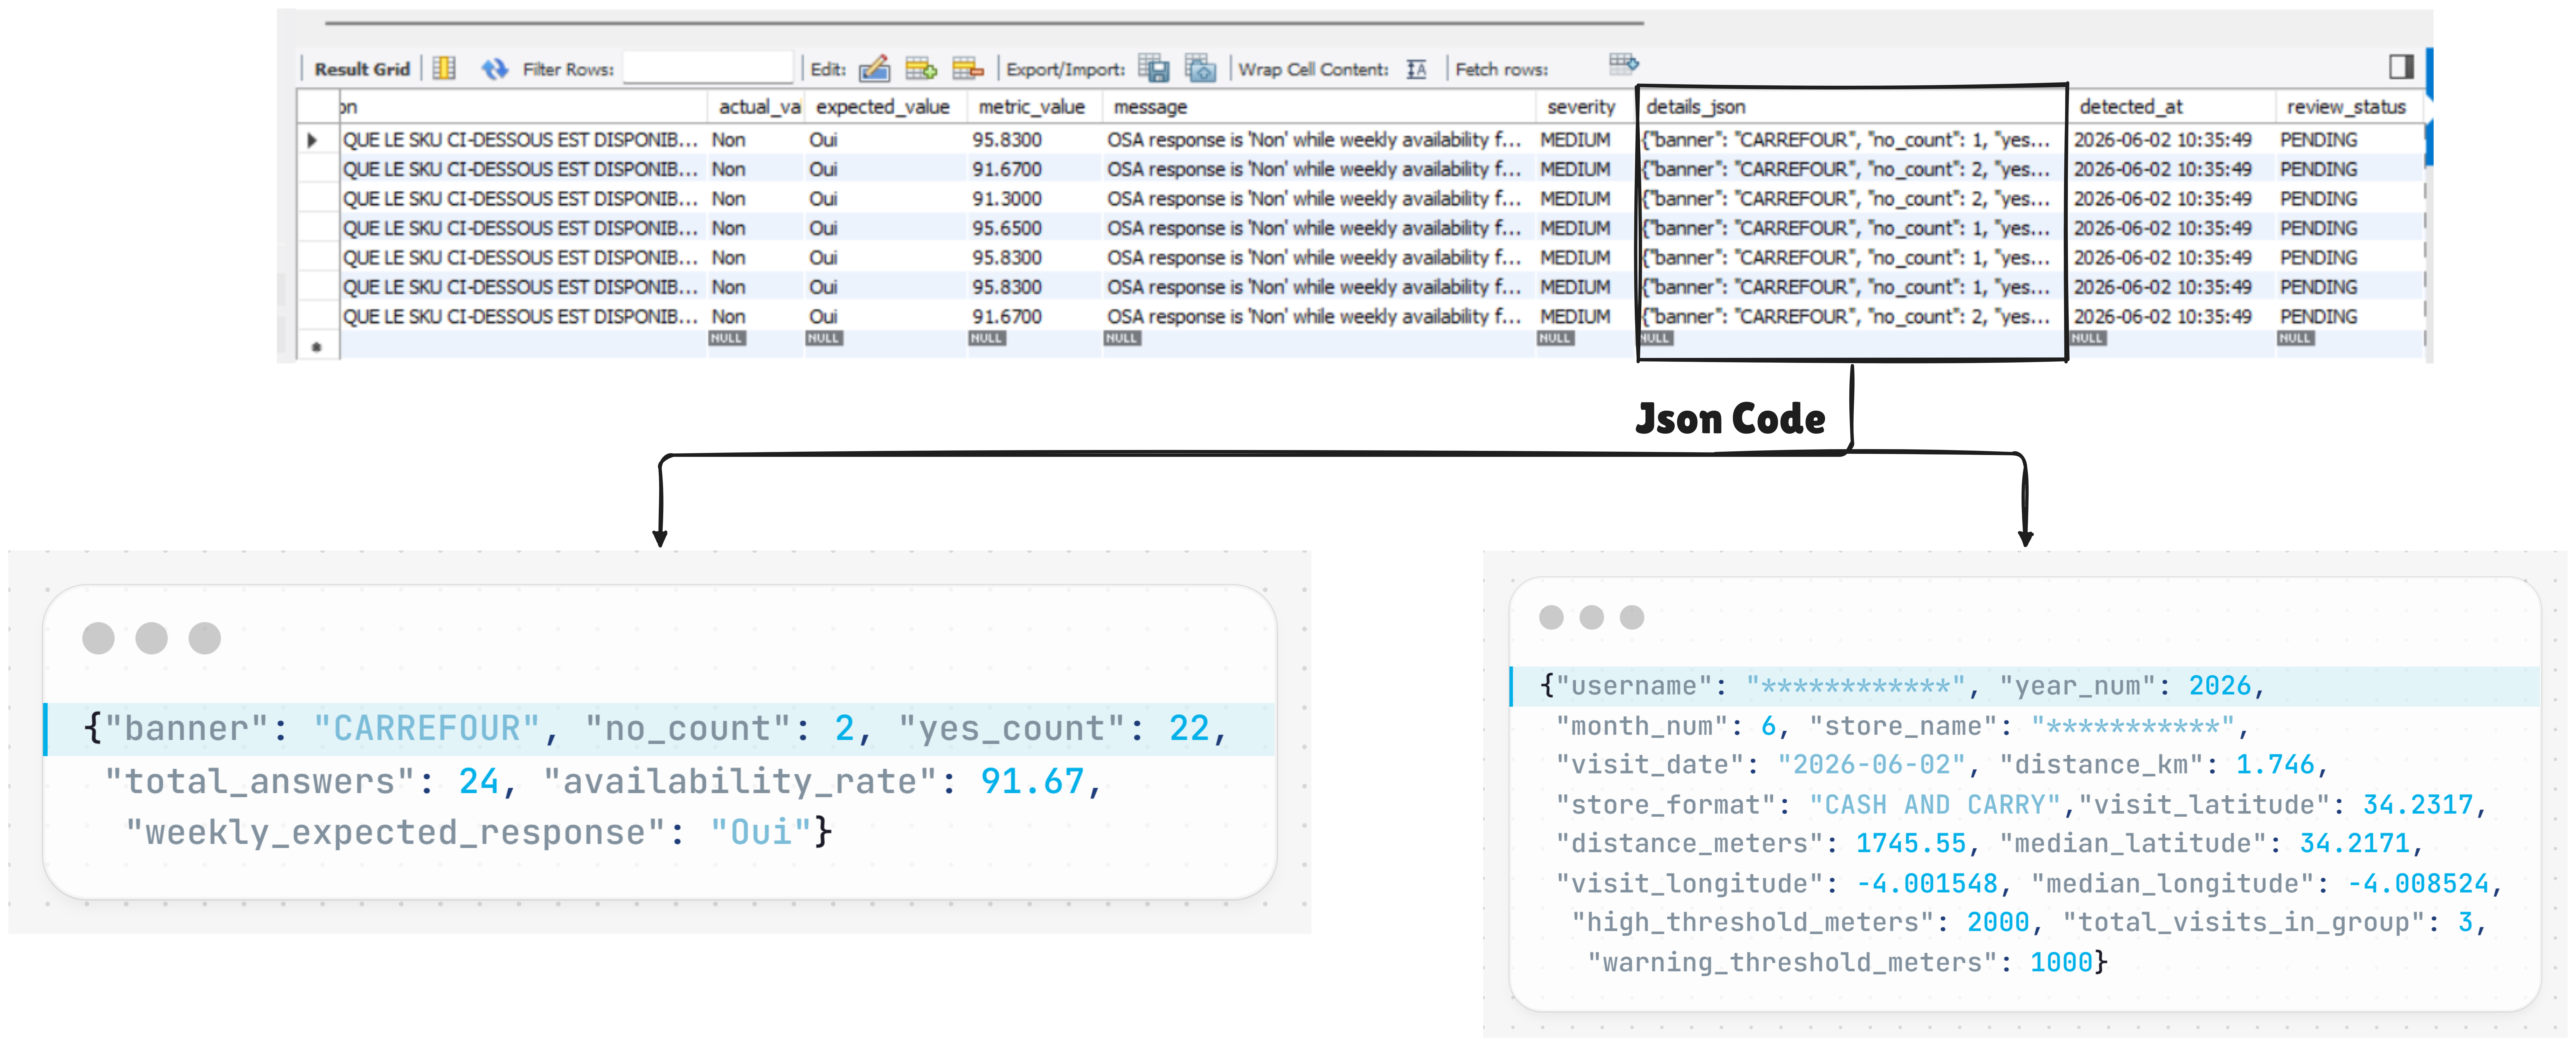
\includegraphics[width=1\textwidth]{figures/results/validation_details_json.png}
    \caption{Exemples de détails JSON associés aux situations OSA et GPS détectées}
    \label{fig:validation_details_json}
\end{figure}

La figure \ref{fig:validation_details_json} montre deux exemples de contenu du champ \dbtable{details\_json}. Pour la règle OSA, ce champ conserve la bannière, le nombre de réponses \textit{Oui} et \textit{Non}, le total des réponses, le taux de disponibilité calculé et la réponse attendue. Pour la règle GPS, il conserve la date de visite, le format du magasin, les coordonnées observées, la position médiane de référence, la distance calculée et les seuils utilisés.

\textbf{Valeur apportée :} cette structure rend les résultats de validation plus exploitables. Les équipes internes ne disposent pas seulement d’un signal à revoir, mais aussi des informations nécessaires pour comprendre pourquoi la situation a été détectée. Le moteur génère ainsi des signaux contextualisés, réservés au back-office interne avant toute décision métier.

\section{Tests des services backend}

Les services backend ont été vérifiés afin de s’assurer que la couche Spring Boot joue correctement son rôle entre la base MySQL et les interfaces de la solution. Les tests réalisés portent sur trois points essentiels : la disponibilité du service, l’exposition des indicateurs de consultation mobile et l’accès interne aux situations détectées par le moteur de validation.

\subsection{Disponibilité du backend}

Le premier contrôle porte sur l’état général du service backend. L’endpoint \url{/api/system/health} permet de vérifier que l’application Spring Boot est démarrée et que la connexion avec la base \dbtable{unilever\_db} est opérationnelle.

\begin{figure}[H]
    \centering
    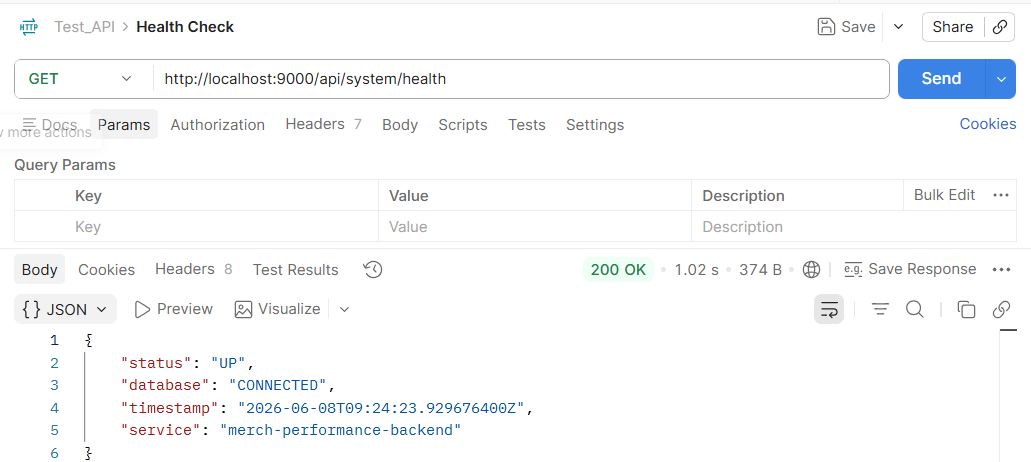
\includegraphics[width=0.90\textwidth]{figures/results/api_system_health.png}
    \caption{Vérification de l’état du service backend}
    \label{fig:api_system_health}
\end{figure}

La figure \ref{fig:api_system_health} confirme que le service est disponible avec un statut \textit{200 OK}. Elle montre également que la connexion à la base de données est active. Ce test constitue donc une vérification de base avant l’analyse des endpoints métier.

\subsection{Test de l’API back-office de validation}

L’endpoint \url{/api/backoffice/validation/issues} a été testé afin de vérifier l’accès aux situations produites par le moteur de validation. Contrairement à l’API mobile, cette API est destinée au portail back-office et expose des informations utiles à la revue interne.

\begin{figure}[H]
    \centering
    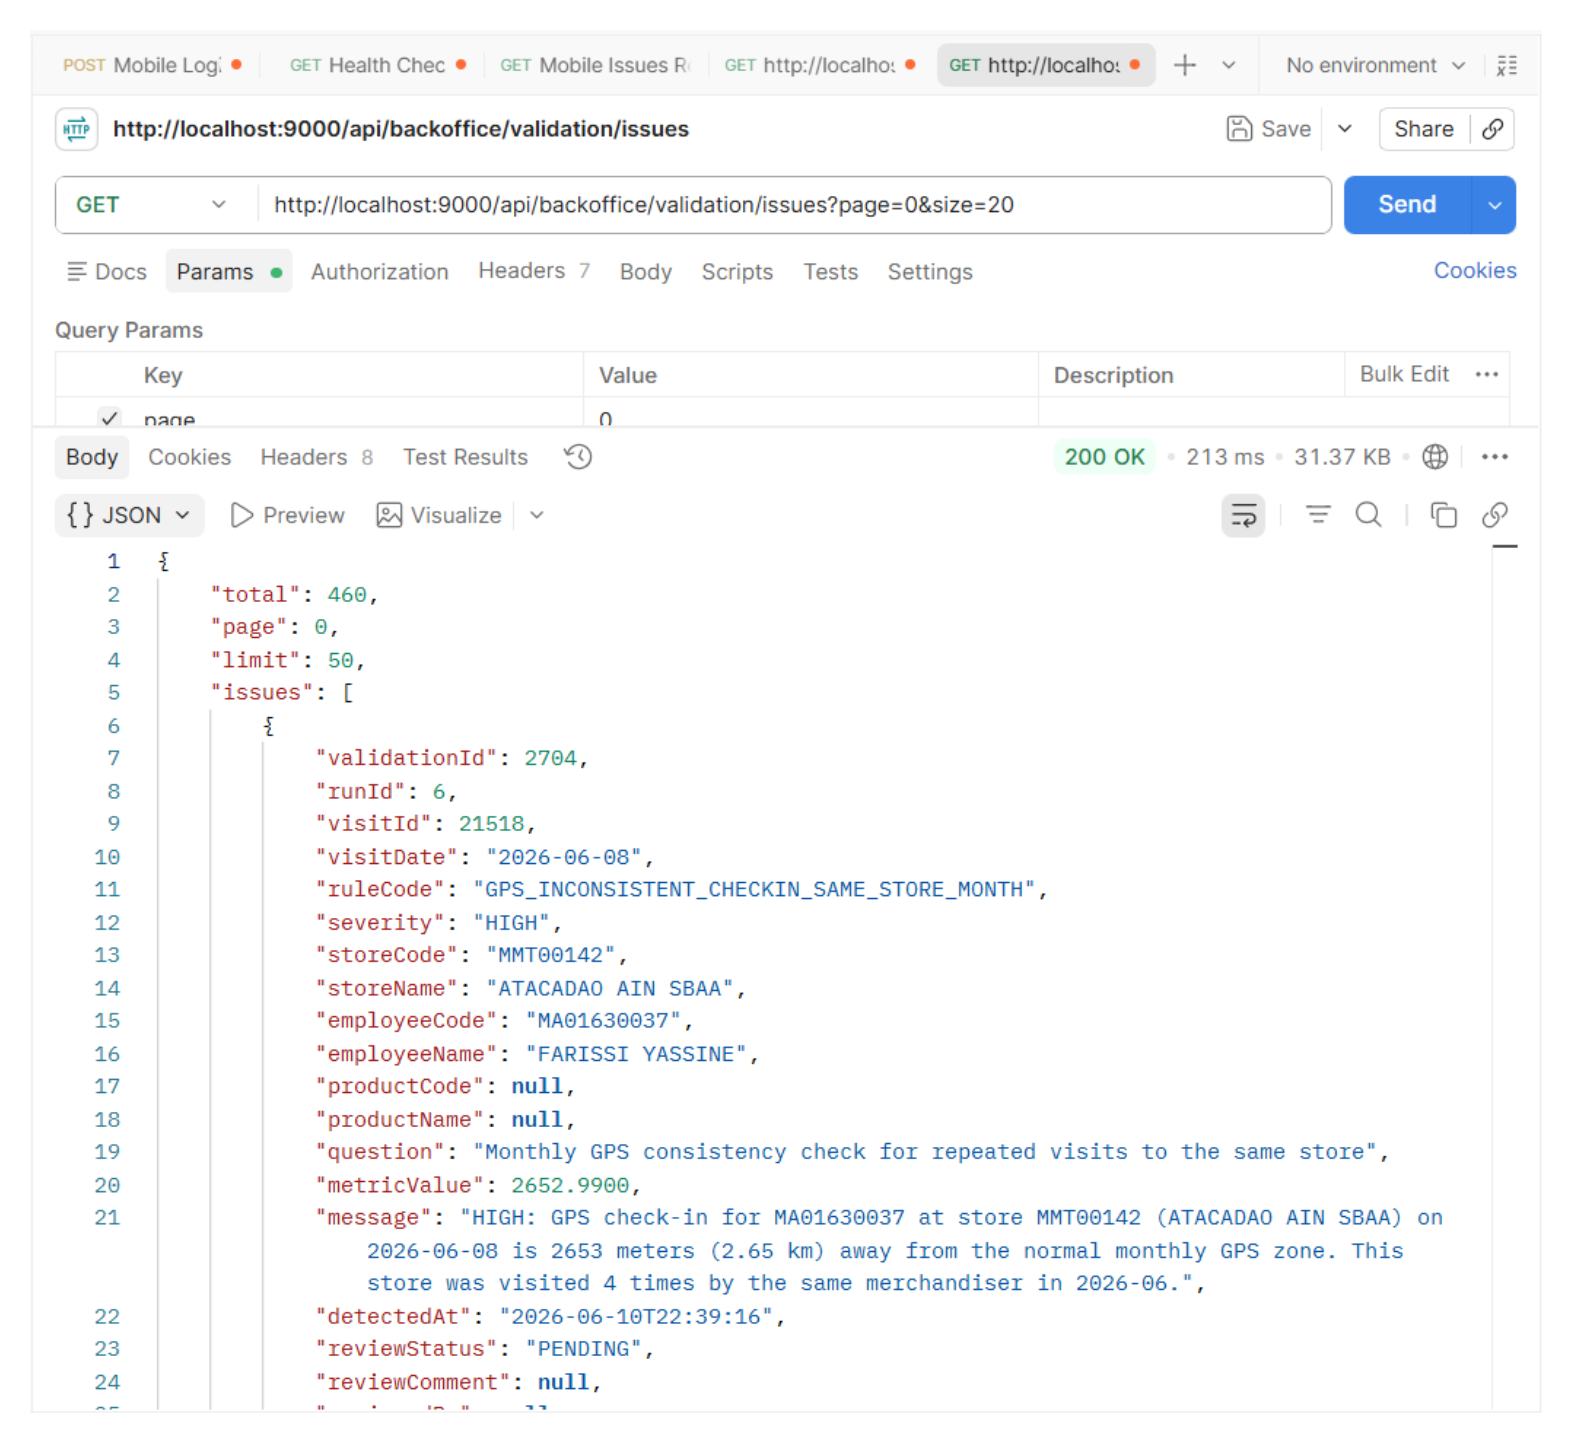
\includegraphics[width=0.95\textwidth]{figures/results/api_backoffice_validation_test.png}
    \caption{Test de l’API back-office \url{/api/backoffice/validation/issues}}
    \label{fig:api_backoffice_validation_test}
\end{figure}

La figure \ref{fig:api_backoffice_validation_test} montre que l’API back-office retourne des données plus détaillées, telles que la règle appliquée, le magasin concerné, le merchandiser, le message de validation, la sévérité et le statut de revue. Ces informations sont nécessaires pour l’analyse interne, mais elles ne sont pas exposées dans l’application mobile.


\subsection{Test de l’API mobile de consultation}

L’endpoint \url{/api/mobile/overview} a été testé afin de vérifier l’exposition des indicateurs destinés à l’application mobile. Cette API retourne une vision synthétique de l’exécution terrain, sous forme d’indicateurs agrégés exploitables par le superviseur côté client.

\begin{figure}[H]
    \centering
    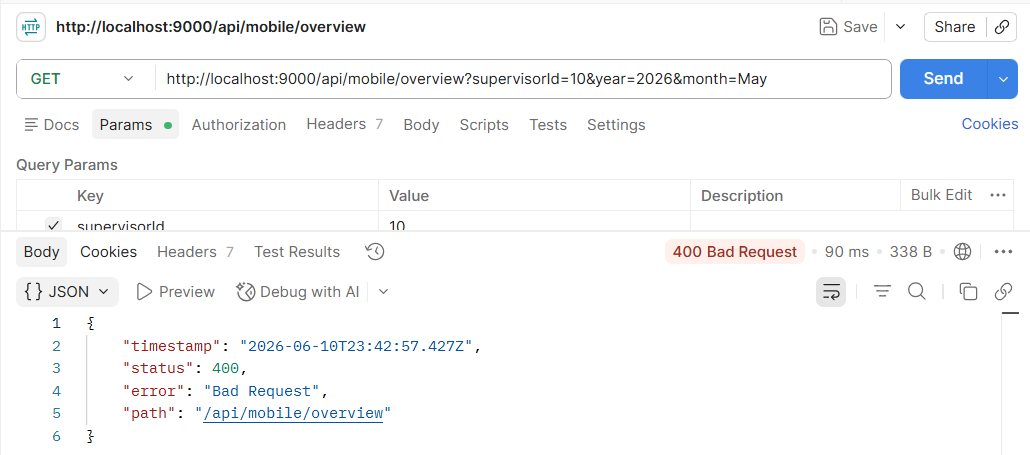
\includegraphics[width=1\textwidth]{figures/results/api_mobile_overview_test.png}
    \caption{Test de l’API mobile \url{/api/mobile/overview}}
    \label{fig:api_mobile_overview_test}
\end{figure}

La réponse obtenue confirme que l’API mobile expose des données de consultation : couverture, visites planifiées, visites réalisées, déviation, indicateurs OSA/SOS et merchandisers actifs. Elle ne retourne pas les règles de validation, les messages d’anomalie ou les statuts de revue interne. Ce comportement confirme la séparation entre consultation mobile et contrôle interne.

\subsection{Interprétation des tests backend}

Les tests réalisés montrent que la couche backend ne se limite pas à lire les tables MySQL et à les retourner telles quelles. Elle joue un rôle de filtre fonctionnel selon l’usage visé. Les données de consultation sont exposées à l’application mobile, tandis que les données sensibles liées à la validation restent réservées au back-office.

Cette séparation améliore la lisibilité et la sécurité fonctionnelle de la solution. Le superviseur côté client accède à des indicateurs simples et exploitables, alors que l’utilisateur back-office dispose des informations nécessaires pour analyser les situations détectées. Ainsi, les tests confirment que l’architecture API respecte la séparation entre consultation opérationnelle et revue interne.

\newpage

\section{Résultats des tableaux de bord Power BI}

Les tableaux de bord Power BI constituent la couche d’analyse décisionnelle de la solution. Leur rôle est de transformer les données centralisées dans MySQL en indicateurs lisibles pour le management, afin de faciliter le suivi de l’exécution terrain et l’identification des priorités d’action.

\subsection{Dashboard exécutif}

La figure \ref{fig:powerbi_executive_dashboard} présente le dashboard exécutif construit pour la période du 1\textsuperscript{er} au 13 mai 2026.

\begin{figure}[H]
    \centering
    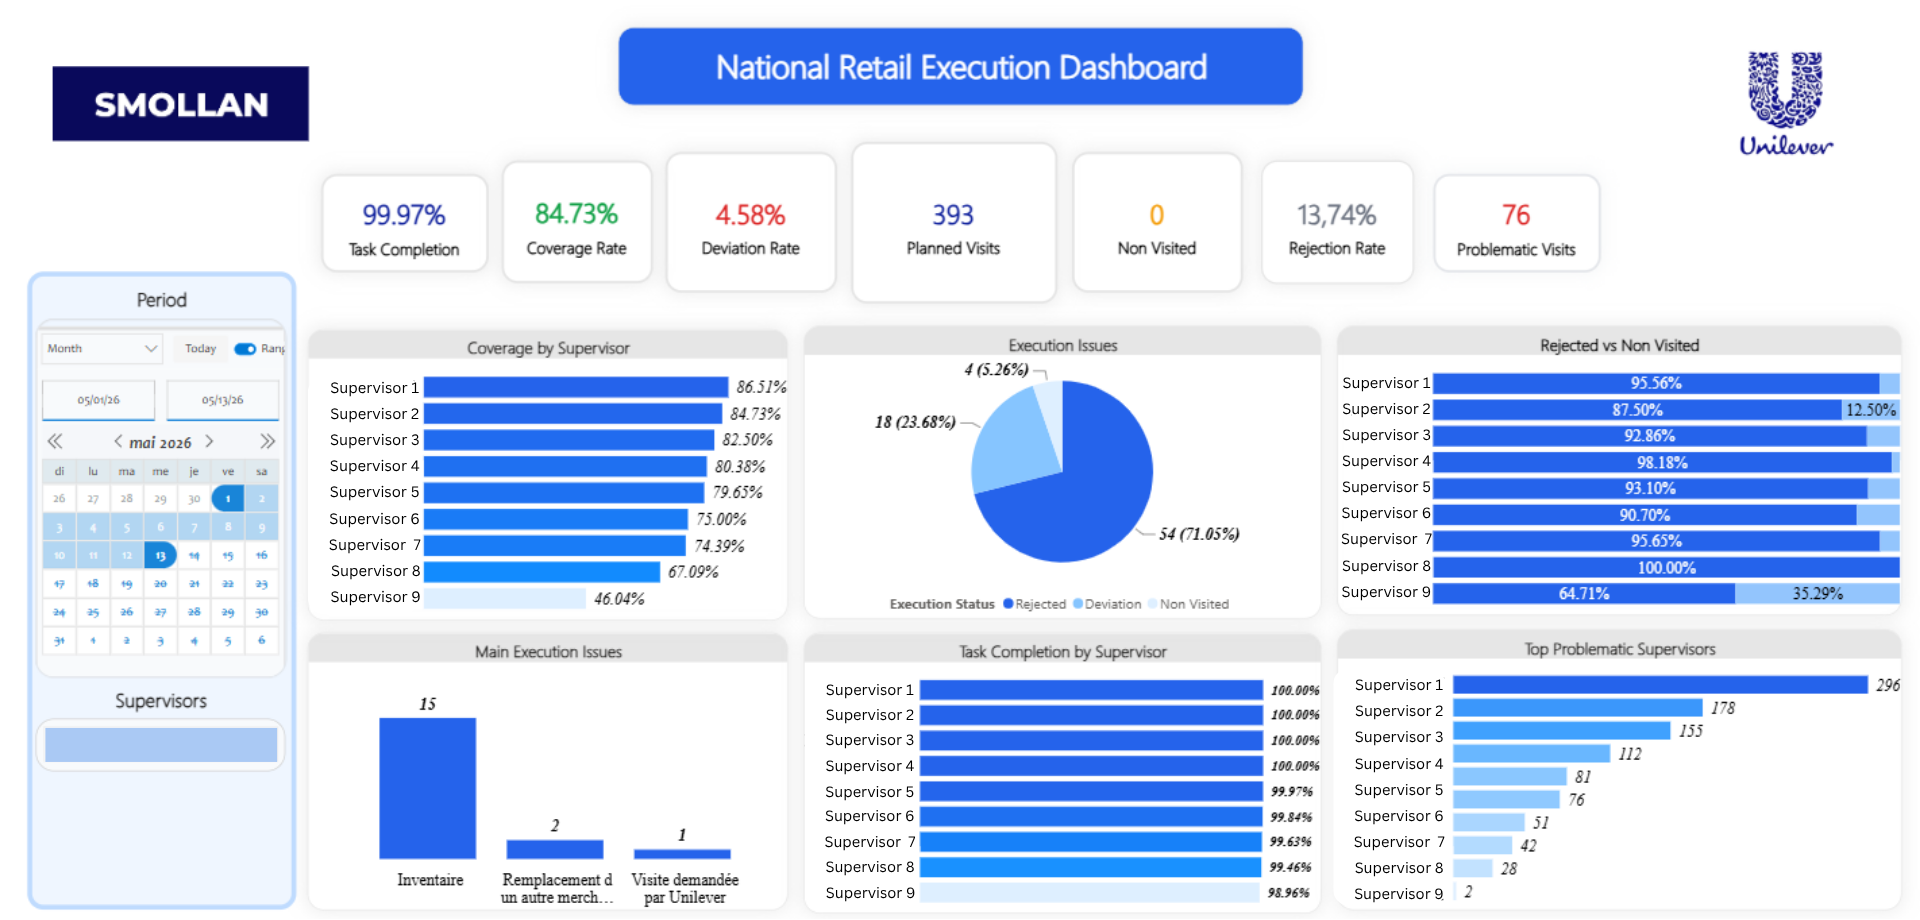
\includegraphics[width=1\textwidth]{figures/results/powerbi_executive_dashboard.png}
    \caption{Dashboard exécutif de suivi national de l’exécution terrain}
    \label{fig:powerbi_executive_dashboard}
\end{figure}

Le dashboard exécutif fournit une vision globale de l’exécution terrain. Il permet de suivre la couverture, les visites problématiques, les rejets, les déviations et les écarts entre superviseurs. Dans l’exemple présenté, la couverture globale atteint \textbf{84,73\%}, avec \textbf{76 visites problématiques}. Les rejets représentent la catégorie dominante des problèmes, avec \textbf{54 cas}, soit \textbf{71,05\%} des visites problématiques.

\textbf{Interprétation :} cette vue permet d’identifier rapidement les priorités de pilotage. Le management peut repérer les périmètres sous la moyenne, suivre les superviseurs présentant les plus grands écarts et orienter l’analyse vers les causes principales de rejet ou de déviation.

\subsection{Dashboard Merchandiser Performance Intelligence}

La figure \ref{fig:powerbi_merchandiser_performance} présente un exemple du dashboard \textit{Merchandiser Performance Intelligence}. Cette vue est orientée vers l’analyse individuelle d’un merchandiser GT sélectionné.

\begin{figure}[H]
    \centering
    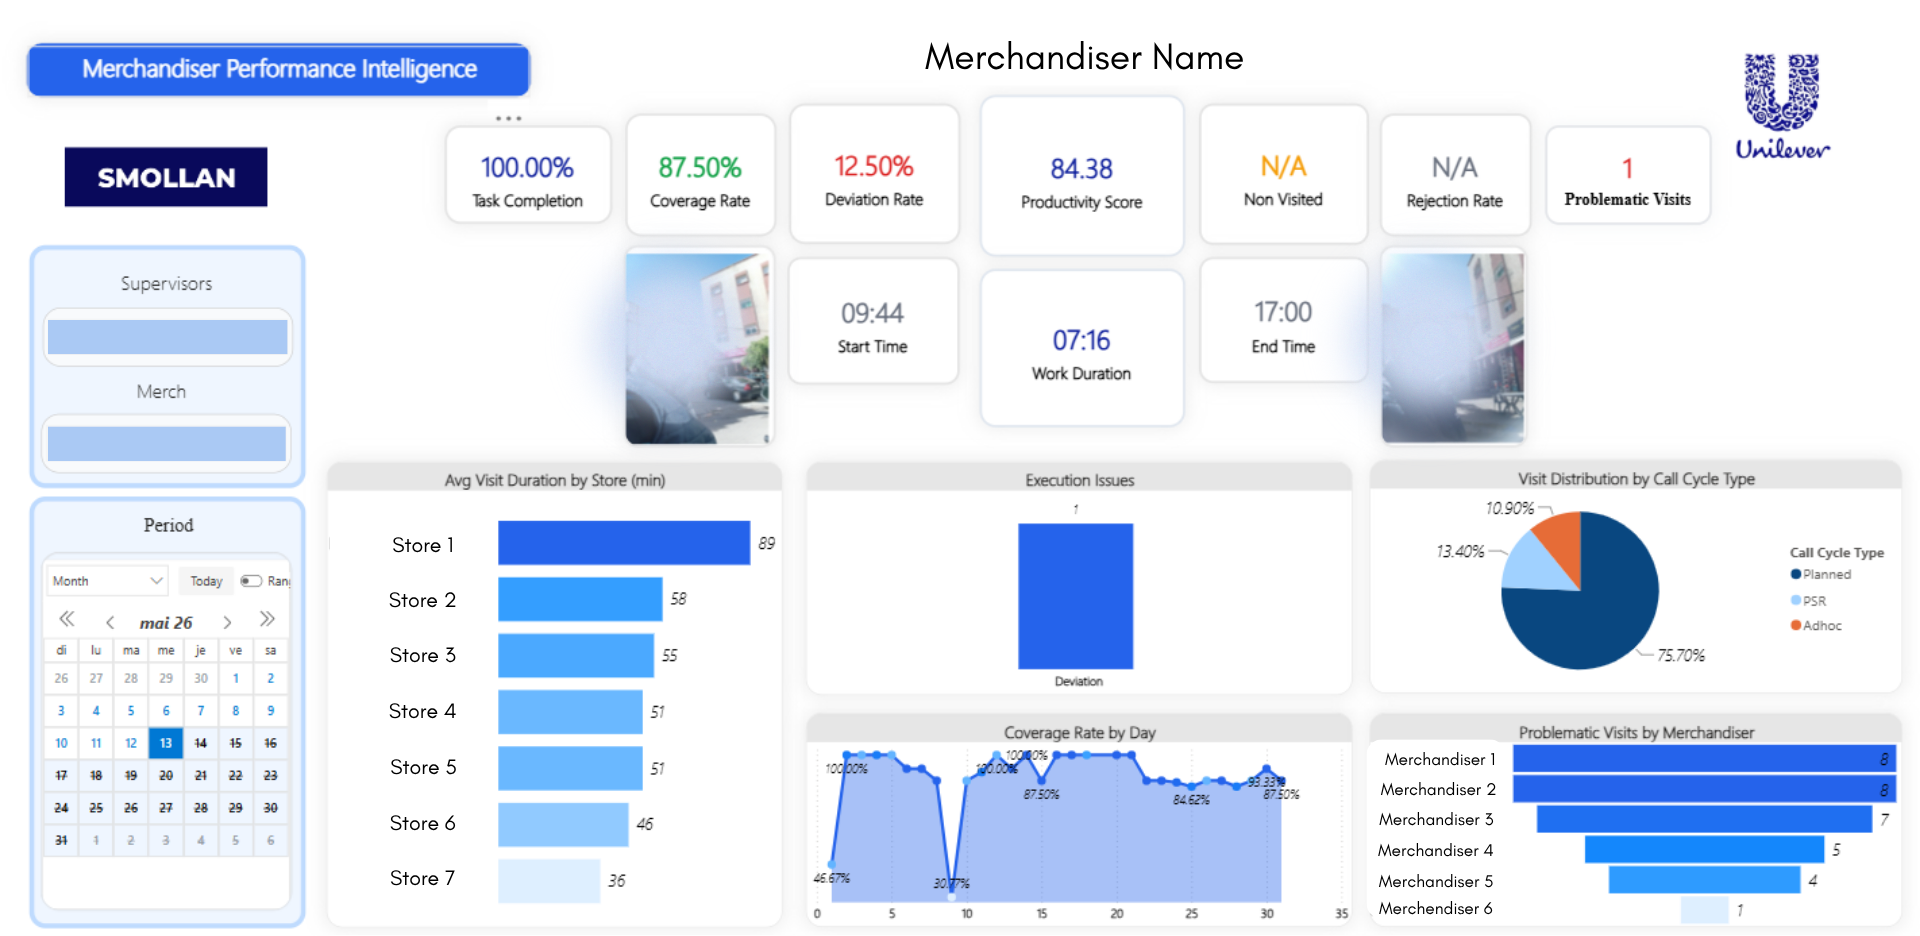
\includegraphics[width=1\textwidth]{figures/results/powerbi_merchandiser_performance.png}
    \caption{Dashboard d’analyse de la performance d’un merchandiser GT}
    \label{fig:powerbi_merchandiser_performance}
\end{figure}

Ce dashboard permet d’analyser la performance d’un merchandiser à partir de plusieurs dimensions : couverture, déviation, productivité, durée de travail, durée moyenne par magasin et type de visite. Dans l’exemple présenté, le merchandiser affiche une couverture GT de \textbf{87,50\%}, un taux de déviation de \textbf{12,50\%} et un score de productivité de \textbf{84,38}.

\textbf{Interprétation :} cette vue permet de passer d’un suivi global à une analyse individuelle. Elle aide à repérer les merchandisers nécessitant un suivi plus rapproché, les magasins demandant plus de temps et les écarts éventuels entre visites planifiées, visites adhoc et visites en déviation.

\subsection{Apport décisionnel pour le management}

L’apport principal de Power BI est de transformer les données centralisées en support d’aide à la décision. Au lieu d’examiner plusieurs fichiers Excel séparés, le management dispose d’une lecture consolidée permettant d’identifier les points d’attention : couverture faible, rejets dominants, écarts entre superviseurs, déviations individuelles et magasins nécessitant un suivi spécifique.

Ainsi, Power BI ne constitue pas seulement une couche de visualisation. Il permet de passer d’un indicateur global à une action de suivi plus ciblée, ce qui renforce l’approche data-driven de la solution.

\newpage

\section{Résultats des interfaces applicatives}

\subsection{Application mobile de consultation côté client}

L’application mobile constitue l’interface de consultation destinée aux superviseurs côté client. Elle permet d’accéder rapidement aux informations essentielles de l’exécution terrain : couverture, visites réalisées, déviations, merchandisers, magasins assignés et détails des tâches effectuées. Son rôle est de restituer les résultats opérationnels de manière simple, sans exposer les informations internes du moteur de validation.

La figure \ref{fig:mobile_login_dashboard} présente l’écran de connexion et le tableau de bord principal. L’accès se fait par email, ce qui permet d’associer l’utilisateur à son périmètre de consultation. Le tableau de bord fournit ensuite une synthèse directe de l’exécution sur la période sélectionnée.

\begin{figure}[H]
    \centering
    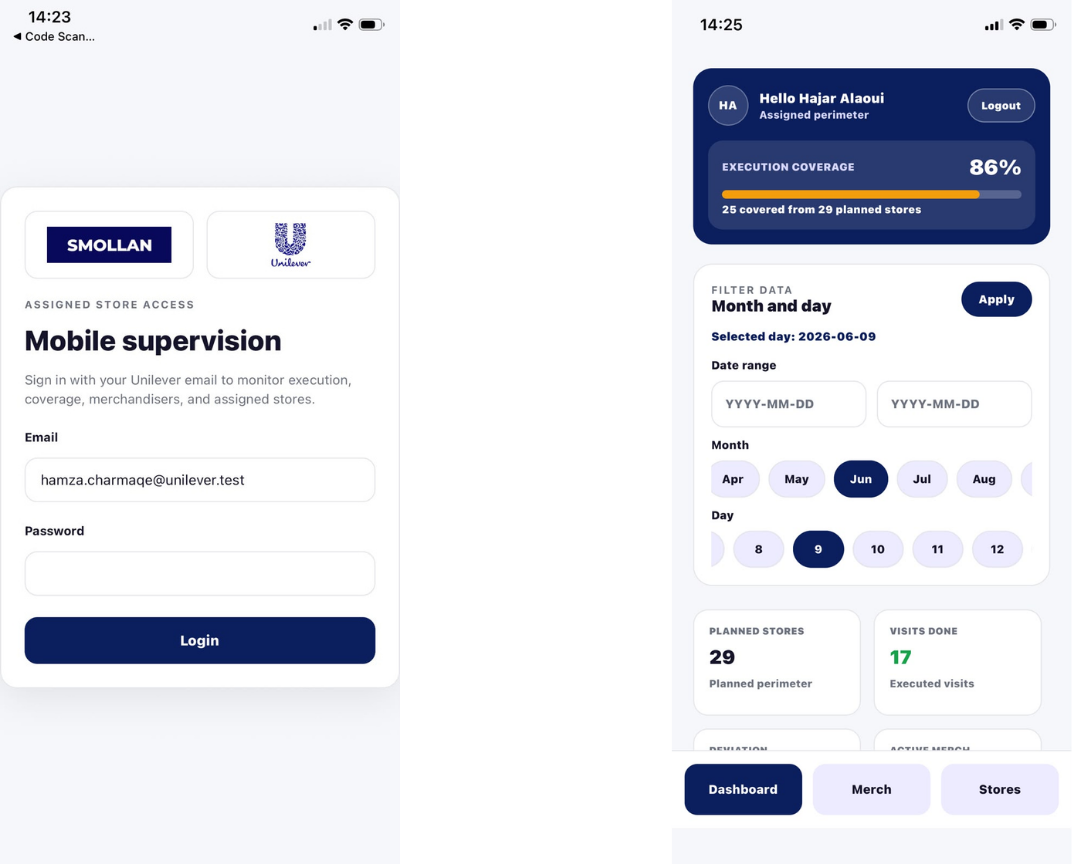
\includegraphics[width=0.95\textwidth]{figures/mobile/mobile_login_dashboard.png}
    \caption{Connexion et tableau de bord de consultation mobile côté client}
    \label{fig:mobile_login_dashboard}
\end{figure}

Dans l’exemple présenté, le tableau de bord indique une couverture d’exécution de \textbf{86\%}, correspondant à \textbf{25 magasins couverts sur 29 magasins planifiés}. Cette information permet au superviseur d’évaluer rapidement l’avancement de son périmètre.

\Needspace{0.65\textheight}
La figure \ref{fig:mobile_merch_execution} illustre le suivi de l’exécution par merchandiser. Cette vue permet de consulter les merchandisers rattachés au périmètre, avec leurs magasins planifiés, leurs visites exécutées et leurs visites en déviation.

\begin{figure}[H]
    \centering
    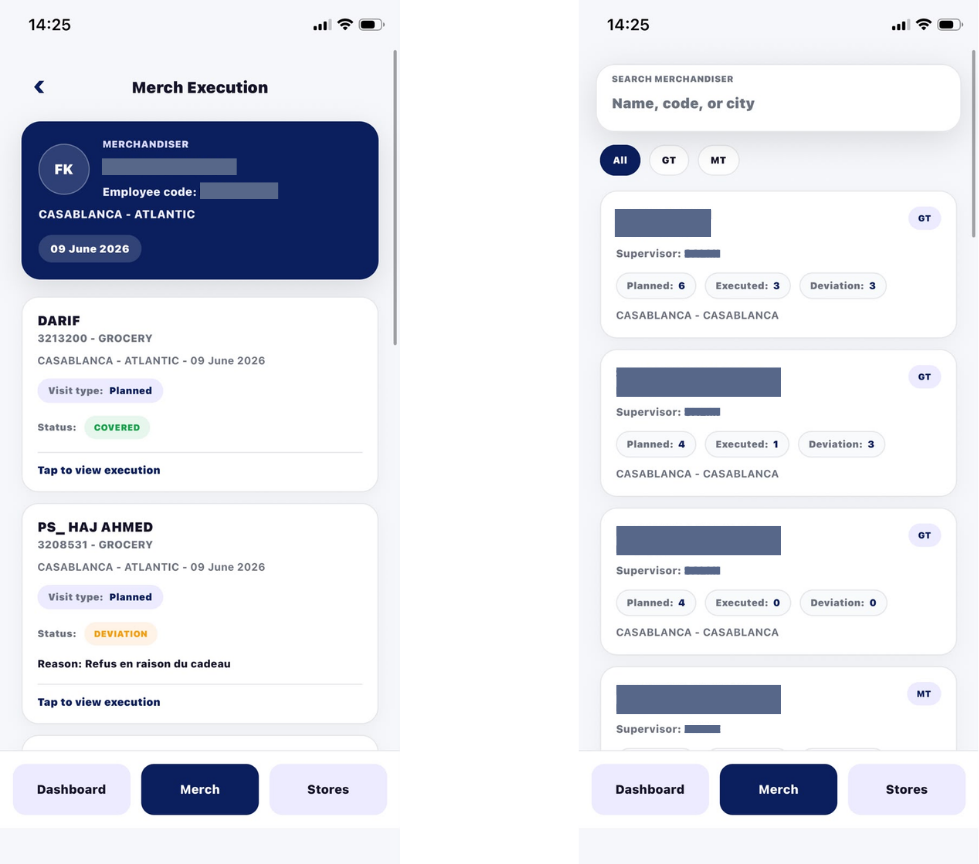
\includegraphics[width=0.95\textwidth]{figures/mobile/mobile_merch_execution.png}
    \caption{Suivi de l’exécution par merchandiser dans l’application mobile}
    \label{fig:mobile_merch_execution}
\end{figure}

Cette organisation facilite le passage d’une lecture globale à une lecture plus ciblée. Le superviseur peut identifier les merchandisers nécessitant un suivi particulier, puis accéder aux magasins associés.

\Needspace{0.65\textheight}
La figure \ref{fig:mobile_store_consultation} présente la consultation des magasins selon deux modes complémentaires : une vue cartographique et une vue liste. La carte facilite le repérage géographique des points de vente, tandis que la liste permet une lecture détaillée par magasin.

\begin{figure}[H]
    \centering
    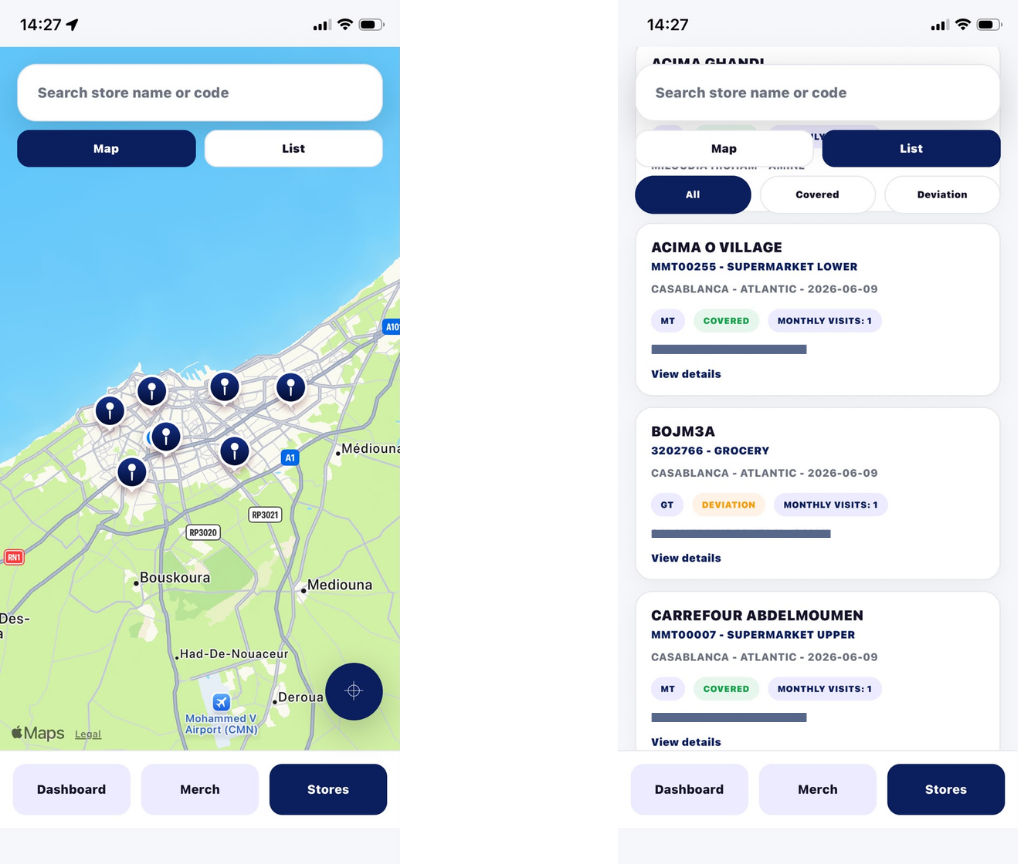
\includegraphics[width=0.95\textwidth]{figures/mobile/mobile_store_consultation.png}
    \caption{Consultation des magasins en mode carte et en mode liste}
    \label{fig:mobile_store_consultation}
\end{figure}

Les filtres de statut, notamment \textit{Covered} et \textit{Deviation}, permettent d’identifier rapidement les magasins couverts et ceux nécessitant une attention particulière.

\Needspace{0.65\textheight}
La figure \ref{fig:mobile_tasks_overview} montre la vue détaillée des tâches associées à une visite. Cette page regroupe les éléments de preuve et les résultats opérationnels : horaires de check-in et check-out, planogramme, indicateurs OSA et SOS, détails par catégorie et éléments de qualité lorsqu’ils sont disponibles.

\begin{figure}[H]
    \centering
    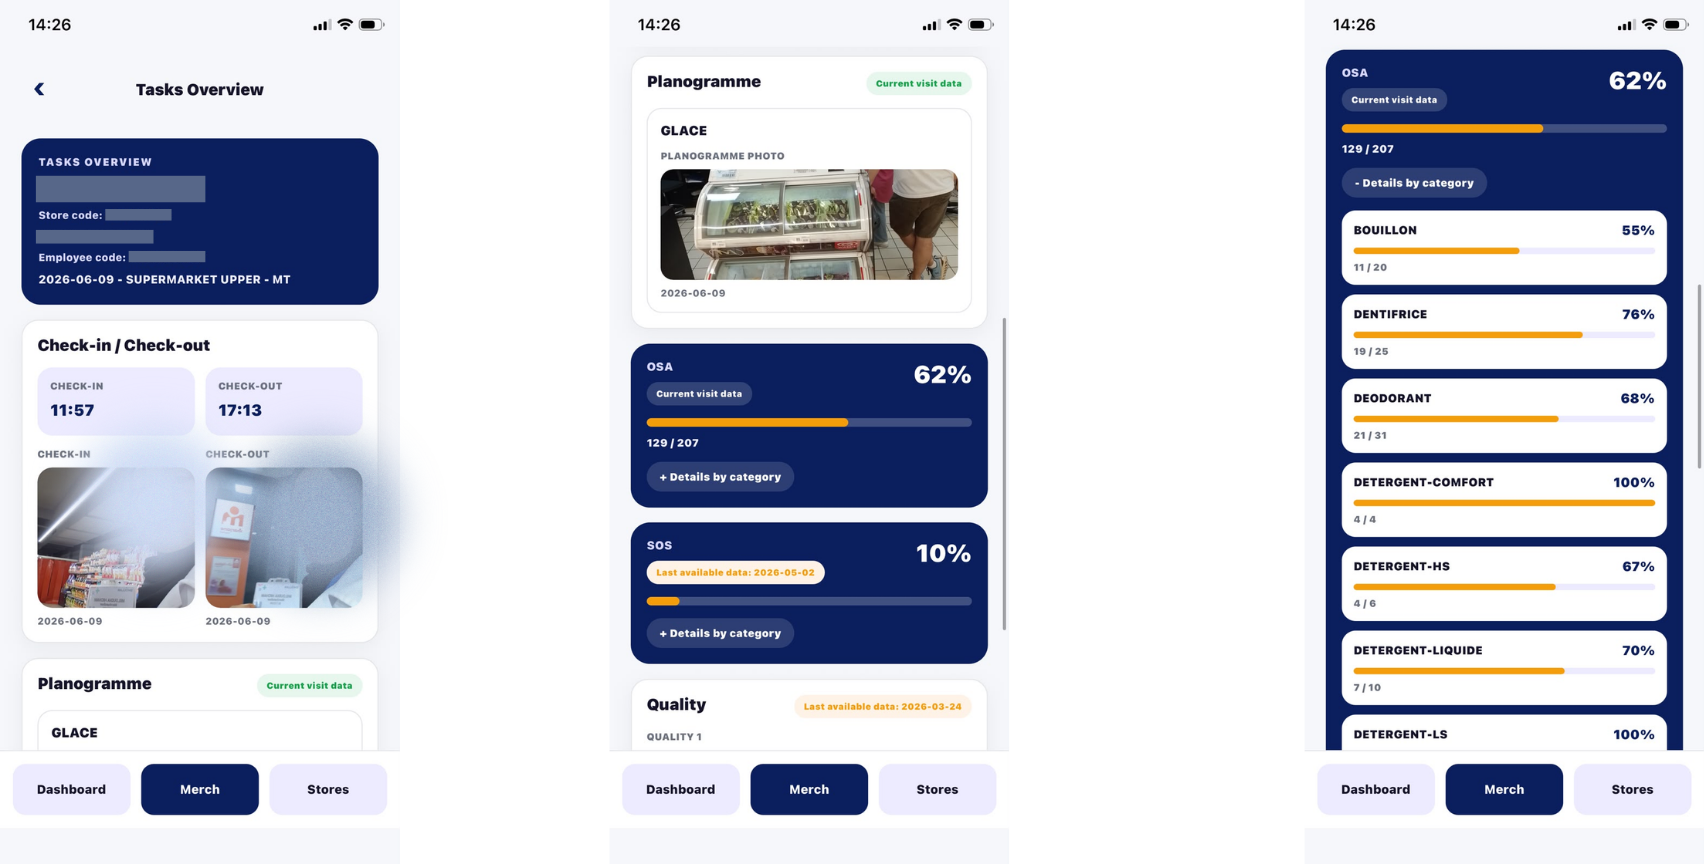
\includegraphics[width=0.95\textwidth]{figures/mobile/mobile_tasks_overview.png}
    \caption{Vue détaillée des tâches et preuves d’exécution terrain}
    \label{fig:mobile_tasks_overview}
\end{figure}

Cette vue relie les indicateurs à des éléments concrets d’exécution terrain. Elle permet de consulter les résultats de visite et les preuves associées, tout en conservant une interface orientée consultation.

\textbf{Valeur apportée :} l’application mobile réduit la dépendance aux rapports Excel partagés et facilite l’accès aux informations de terrain. Elle expose les données utiles au suivi côté client : couverture, exécution, statuts de visite, OSA, SOS, planogramme, qualité et preuves d’exécution. En revanche, les règles de validation, les messages d’anomalie, les statuts de revue et les commentaires internes restent réservés au back-office.

\subsection{Portail back-office de validation}

Le portail back-office constitue l’espace interne de suivi et de revue des situations détectées par le moteur de validation. Contrairement à l’application mobile, qui est orientée consultation côté client, le back-office expose les informations nécessaires au traitement interne : règle appliquée, magasin concerné, merchandiser, type de situation, statut de revue et action possible.

La figure \ref{fig:backoffice_problem_overview_mt_osa} présente la vue \textit{Problem Stores Overview} filtrée sur le périmètre MT--OSA. Cette vue regroupe les situations détectées par magasin afin de faciliter la priorisation des cas à analyser.

\begin{figure}[H]
    \centering
    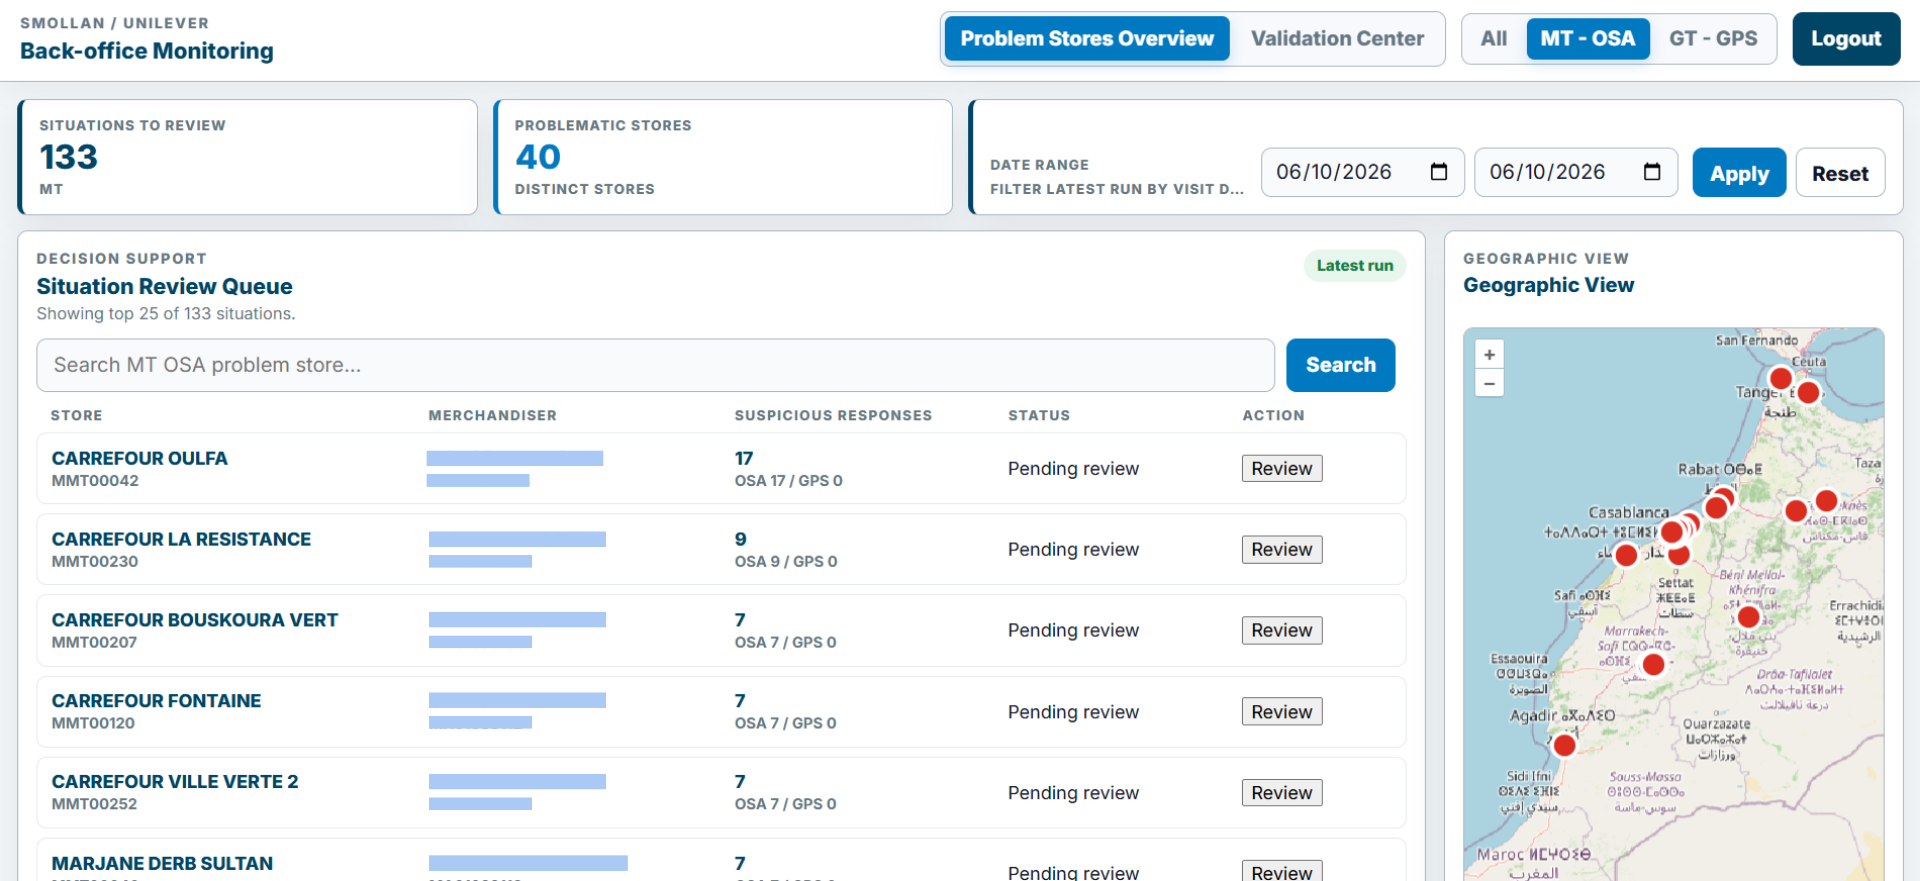
\includegraphics[width=1\textwidth]{figures/results/backoffice_problem_overview_mt_osa.png}
    \caption{Vue back-office des magasins problématiques pour le périmètre MT--OSA}
    \label{fig:backoffice_problem_overview_mt_osa}
\end{figure}

Dans l’exemple affiché, le back-office identifie \textbf{133 situations à revoir}, regroupées sur \textbf{40 magasins distincts}. Cette agrégation évite de traiter chaque ligne de validation de manière isolée et permet de concentrer l’analyse sur les magasins les plus concernés.

La figure \ref{fig:backoffice_problem_overview_gt_gps} montre la même logique appliquée au périmètre GT--GPS. Dans ce cas, l’interface met en évidence une situation GPS à revoir pour un magasin distinct.

\begin{figure}[H]
    \centering
    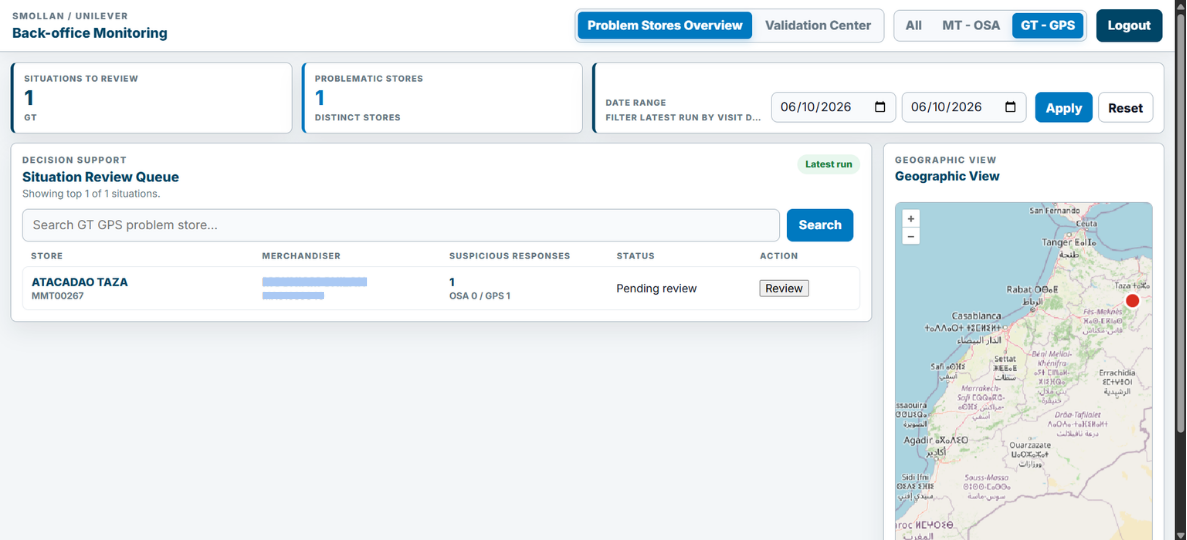
\includegraphics[width=1\textwidth]{figures/results/backoffice_problem_overview_gt_gps.png}
    \caption{Vue back-office des magasins problématiques pour le périmètre GT--GPS}
    \label{fig:backoffice_problem_overview_gt_gps}
\end{figure}

Cette séparation entre MT--OSA et GT--GPS reflète la logique métier retenue dans la solution. Les magasins MT sont principalement suivis à travers les anomalies OSA, tandis que les magasins GT sont suivis à travers la cohérence GPS. Le back-office permet donc de filtrer les situations selon le type de contrôle le plus pertinent pour chaque périmètre.

La figure \ref{fig:backoffice_validation_center} présente le \textit{Validation Center}. Cette vue donne accès aux détections détaillées et permet de consulter une situation sélectionnée avec son contexte.

\begin{figure}[H]
    \centering
    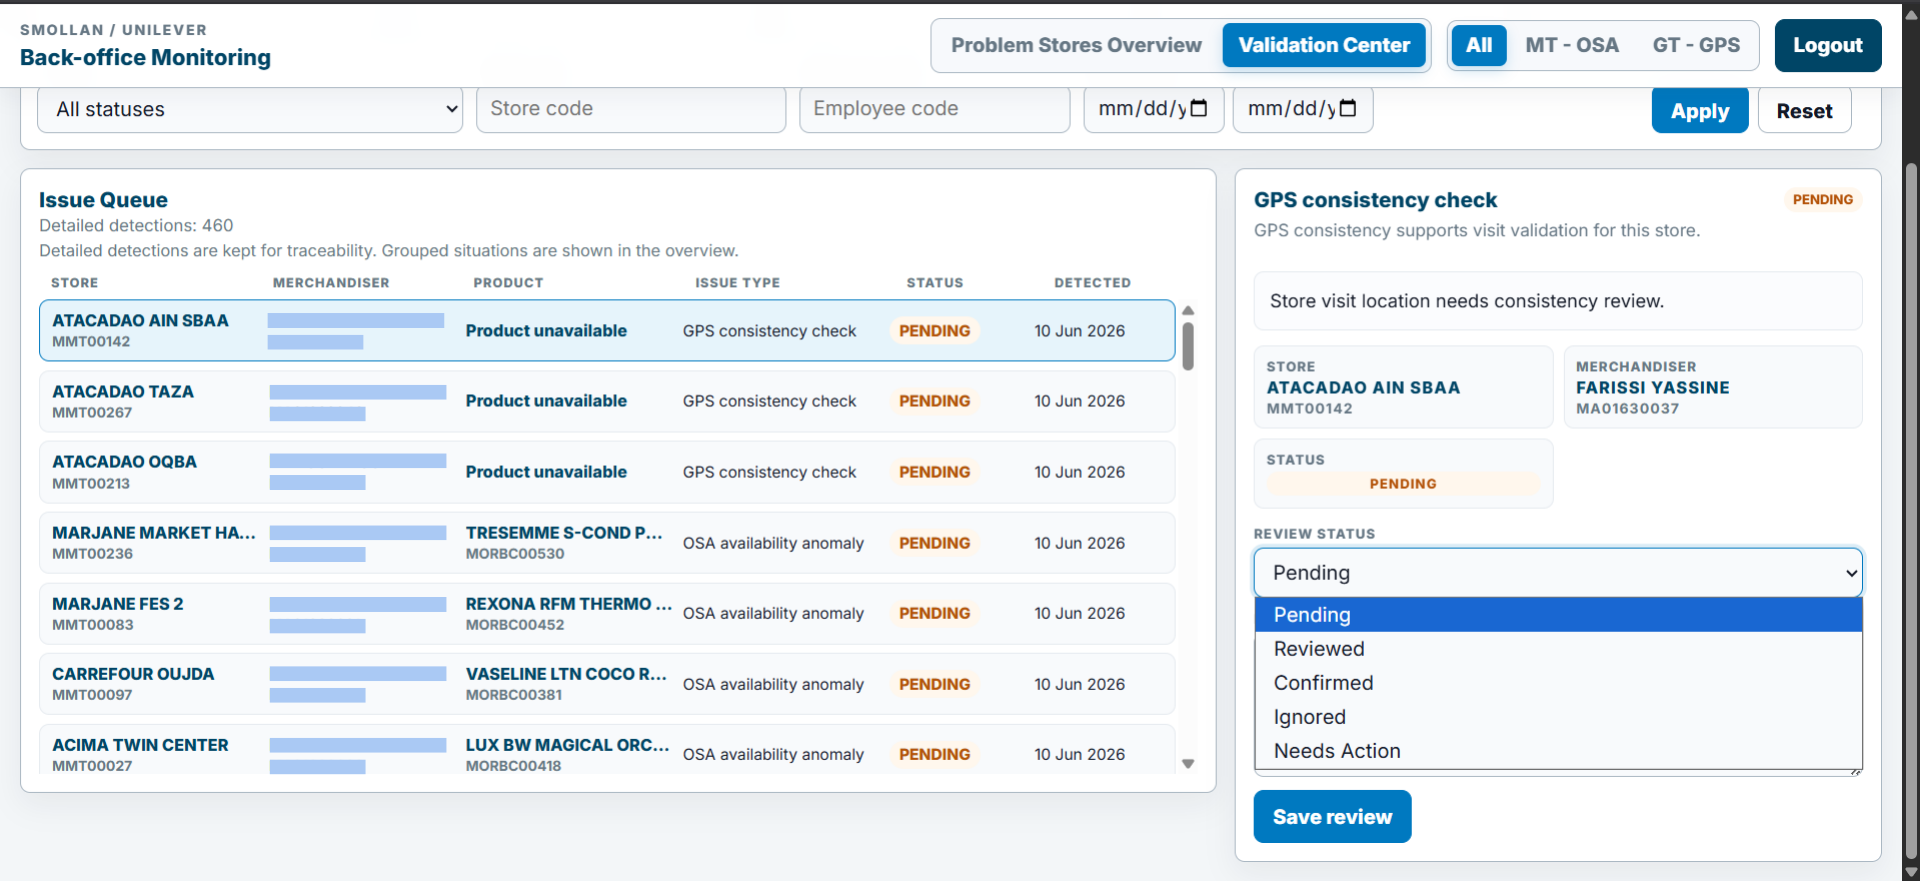
\includegraphics[width=1\textwidth]{figures/results/backoffice_validation_center.png}
    \caption{Centre de validation interne des situations détectées}
    \label{fig:backoffice_validation_center}
\end{figure}

Dans l’exemple affiché, le centre de validation contient \textbf{460 détections détaillées}. La partie gauche présente la file des situations détectées, tandis que la partie droite affiche le détail du cas sélectionné. L’utilisateur interne peut consulter le magasin, le merchandiser, le type de problème, le statut courant et modifier le statut de revue.

\textbf{Valeur apportée :} le back-office transforme les résultats du moteur de validation en une file de travail organisée. La vue \textit{Problem Stores Overview} permet de prioriser les magasins les plus concernés, tandis que le \textit{Validation Center} permet de descendre au niveau de la détection détaillée. Cette organisation évite de traiter les résultats comme de simples lignes techniques et les rend exploitables pour la revue interne.

Ainsi, le back-office complète l’application mobile sans la remplacer. L’application mobile fournit une consultation simple côté client, alors que le back-office conserve les informations sensibles nécessaires à l’analyse interne avant toute décision métier.

\section{Synthèse de l’apport de la solution}

Après avoir présenté les résultats techniques, les tests et les interfaces de la solution, cette section synthétise l’apport global du projet. L’objectif est de montrer comment la solution répond aux limites du processus initial et améliore la structuration, l’exploitation et le suivi des données merchandising.

\subsection{Comparaison avant/après}

Le tableau \ref{tab:comparaison_avant_apres_solution} présente une comparaison synthétique entre le fonctionnement initial et l’approche proposée.

\begin{table}[H]
\centering
\caption{Comparaison entre le processus initial et la solution proposée}
\label{tab:comparaison_avant_apres_solution}
\renewcommand{\arraystretch}{1.15}
\setlength{\tabcolsep}{4pt}
\small
\begin{tabular}{L{4.2cm} L{4.8cm} L{4.8cm}}
\toprule
\textbf{Aspect analysé} & \textbf{Avant la solution} & \textbf{Après la solution} \\
\midrule
Exploitation des données & Fichiers Excel séparés et manipulés manuellement & Données centralisées dans MySQL \\
\addlinespace
Temps de préparation & Environ 2h30 pour les reportings internes et client & Exécution automatisée en 9 min 23 s \\
\addlinespace
Traçabilité & Suivi limité des étapes de traitement & Runs, statuts et logs Prefect \\
\addlinespace
Contrôles métier & Vérifications manuelles sur OSA et GPS & Règles de validation automatisées \\
\addlinespace
Consultation côté client & Dépendance aux rapports partagés & Application mobile de consultation \\
\addlinespace
Suivi interne & Analyse dispersée dans les fichiers ou tables & Back-office de revue des situations détectées \\
\addlinespace
Pilotage & Lecture fragmentée par fichier ou rapport & Dashboards Power BI consolidés \\
\bottomrule
\end{tabular}
\end{table}

Cette comparaison montre que la solution ne se limite pas à ajouter des outils techniques autour du processus existant. Elle modifie la logique de travail : les fichiers Excel deviennent une source d’entrée, tandis que MySQL, Prefect, les APIs, Power BI, l’application mobile et le back-office forment une chaîne structurée d’exploitation des données.

\subsection{Apport global de la solution}

L’apport principal du projet réside dans la transformation d’un processus dépendant de fichiers Excel en une solution data-driven structurée. Cette transformation se traduit par plusieurs résultats concrets : réduction du temps de préparation, centralisation des données, traçabilité des traitements, automatisation des premiers contrôles métier et restitution des résultats selon les usages.

Sur le plan technique, la solution met en place une chaîne cohérente allant de l’acquisition des fichiers jusqu’à leur exploitation applicative. Les données sont centralisées dans MySQL, les traitements sont orchestrés dans Prefect et les services backend exposent les informations selon les besoins.

Sur le plan métier, la solution facilite le suivi de l’exécution terrain. Le superviseur côté client dispose d’une application mobile de consultation, les équipes internes disposent d’un back-office pour traiter les situations détectées, et le management dispose de dashboards Power BI pour analyser les indicateurs et orienter les actions de suivi.

\section{Limites et état actuel de la solution}

À la fin du projet, la solution réalisée permet de valider les principaux choix techniques et fonctionnels retenus. Le pipeline Data Engineering est opérationnel, les données sont centralisées dans MySQL, les premiers contrôles métier sont automatisés, les APIs principales ont été testées, et les résultats peuvent être exploités à travers Power BI, l’application mobile et le back-office. L’état actuel correspond donc à une solution fonctionnelle de PFE, capable de démontrer la faisabilité de l’approche proposée.

Cependant, cette version ne doit pas être présentée comme une plateforme totalement industrialisée. La solution a été testée principalement dans un environnement local ; un déploiement serveur ou cloud nécessiterait une configuration plus stable, adaptée à un usage quotidien et à plusieurs utilisateurs. De plus, la gestion des accès pourrait être renforcée par une gestion plus complète des rôles, des sessions et de la traçabilité des actions, notamment pour le portail back-office.

Enfin, certaines évolutions fonctionnelles restent possibles. L’application mobile pourrait intégrer un mode hors ligne ou une synchronisation locale pour mieux répondre aux contraintes terrain. Le moteur de validation pourrait être enrichi par de nouvelles règles métier, et les dashboards Power BI pourraient intégrer davantage d’analyses historiques et comparatives. Ces limites ne remettent pas en cause les résultats obtenus ; elles montrent plutôt que la solution constitue une base fonctionnelle solide et évolutive.

\section{Conclusion}

Ce chapitre a présenté les principaux résultats obtenus après la mise en œuvre de la solution. Les résultats montrent que le projet a permis de passer d’un suivi fortement dépendant des fichiers Excel à une chaîne plus structurée, dans laquelle les données sont centralisées, contrôlées, exposées et restituées selon des usages clairement séparés.

Le premier apport mesurable concerne le pipeline Data Engineering. L’exécution automatisée en 9 minutes et 23 secondes, contre un processus manuel estimé à environ 2h30, montre que l’automatisation réduit fortement le temps de préparation et améliore la traçabilité du traitement.

Les règles OSA et GPS ont permis de transformer un volume important de données terrain en situations ciblées à analyser. Les tests des APIs, les dashboards Power BI, l’application mobile et le back-office confirment également la cohérence globale de la solution. Ainsi, la solution réalisée constitue une base fonctionnelle cohérente pour améliorer le suivi des opérations de merchandising du projet Unilever chez Smollan Morocco.
